% uklad dokumentu
	\documentclass{article}
	\usepackage{xparse}
	\usepackage[margin=2cm]{geometry}
    \usepackage{enumerate} 
	\frenchspacing
    \linespread{1.2}
    \setlength{\parindent}{0pt}

% jezyk polski
	\usepackage[polish]{babel}
	\usepackage[utf8]{inputenc}
	\usepackage{polski}
	\usepackage[T1]{fontenc}
 
% pakiety matematyczne
    \let\lll\undefined
	\usepackage{amssymb}
    \usepackage{amsthm}
	\usepackage{amsmath}
	\usepackage{amsfonts}
	\usepackage{tikz}

% hiperlacza
	\usepackage{hyperref}
	\hypersetup{
		colorlinks,
		citecolor=black,
		filecolor=black,
		linkcolor=black,
		urlcolor=black
	}

% wstawianie zdjec
	\usepackage{graphicx} 
    
% podstawowe informacje
    \title{\textbf{Projekt aplikacji opartej o relacyjną bazę danych} \\ \normalsize{<tu wpisz tytuł>}}
    \author{Jarosław Nigiel, Adam Friedensberg}
    \date{semestr zimowy 2016/2017}

\begin{document}
	\maketitle
    
%    \tableofcontents %%% jeśli potrzebujesz spis treści, odkomentuj linię
    
    \section{Analiza problemu/zagadnienia}
    Zaprezentowana aplikacja ma za zadanie pomóc użytkownikowi w kontrolowaniu miesięcznych wydaktów i przy ustalonym budżecie liczyć, ile pieniędzy pozostało jeszcze dostępnych do końca ustalonego miesiąca rozliczeniowego. Aplikacja nie ma na celu ograniczać użytkownika, lecz stanowić pomoc informacyjną i działać jako historia dokonanych płatności.
    
    \section{Wymagania funkcjonalne}
    Przedstawiona poniżej lista określa najważniejsze możliwości funkcjonalne aplikacji:
    \begin{itemize}
    \item Możliwość zalogowania się, bądź utworzenia nowego konta użytkownika
    \item Zdatność do usunięcia konta z poziomu administratora
    \item Istnienie trzech rodzajów użytkowników: Podstawowych, Premium, Administratorów
    \item Ustalenie miesięcznego budżetu do rozdysponowania przez użytkownika
    \item Wprowadzenie do bazy rekordów o dokonanych płatnościach wraz z ich kosztem (zakupy w sklepie)
    \item Śledzenie historii dokonanych transakcji z dokładną datą wprowadzenia rekordów
    \item Ustalanie aktualnego budżetu na podstawie płatności z bazy
    \item Możliwość sortowania rekordów, w celu wyszukania ceny i ilości zakupionych dóbr, usług
    \item Zdatność do uwzględnienia w rozliczanym budżecie płatności stałych z ustawioną datą realizacji
    \item Ustawianie początku i końca miesiąca rozliczeniowego w aplikacji
    \item Włączenie przez użytkownika opcji liczenia oszczędności, jako pozostałości niewydanego budżetu z poprzednich miesięcy i przeznaczenie ich do konkretnego celu
    \item Możliwość dodania do bazy danych konkretnego sklepu, bądź produktu w celu ich wyszukania w przyszłości bądź wybrania z dostępnej listy przy wprowadzaniu rekordów o transakcjach
    \item Wykorzystanie z bazy danych unikalnej dla użytkownika listy produktów, usług oraz lokalizacji ich nabycia w celu skrócenia czasu wprowadzania rekordów o płatnościach przez klienta
    \item Umożliwienie użytkownikowi opcji "błyskawicznego" dodania rekordu o płatnościach ustawionych jako ulubione, w przypadku czynności wykonywanych z dużą częstotliwością, np. poranna kawa w kawiarni blisko uczelni, miejsca pracy, etc.
    \end{itemize}
    
    \section{Wymagania niefunkcjonalne}
    Gotowa aplikacja będzie spełniała dodatkowe wymagania podane poniżej:
    \begin{itemize}
    \item Zapewnienie bezpieczeństwa związanego z ochroną danych użytkowników
    \item Utrzymanie spójności i stabilności podczas korzystania z programu
    \item Korzystanie z aplikacji poprzez intuicyjny i spełniający swoją rolę interfejs
    \item Zapewnienie przystępnej dla użytkownika wydajności programu
    \item Kontrolowanie niezawodności działania aplikacji wraz z pomocą techniczną
    \end{itemize}
    
    \section{Projekt bazy danych (diagram UML)}
    
    \centering 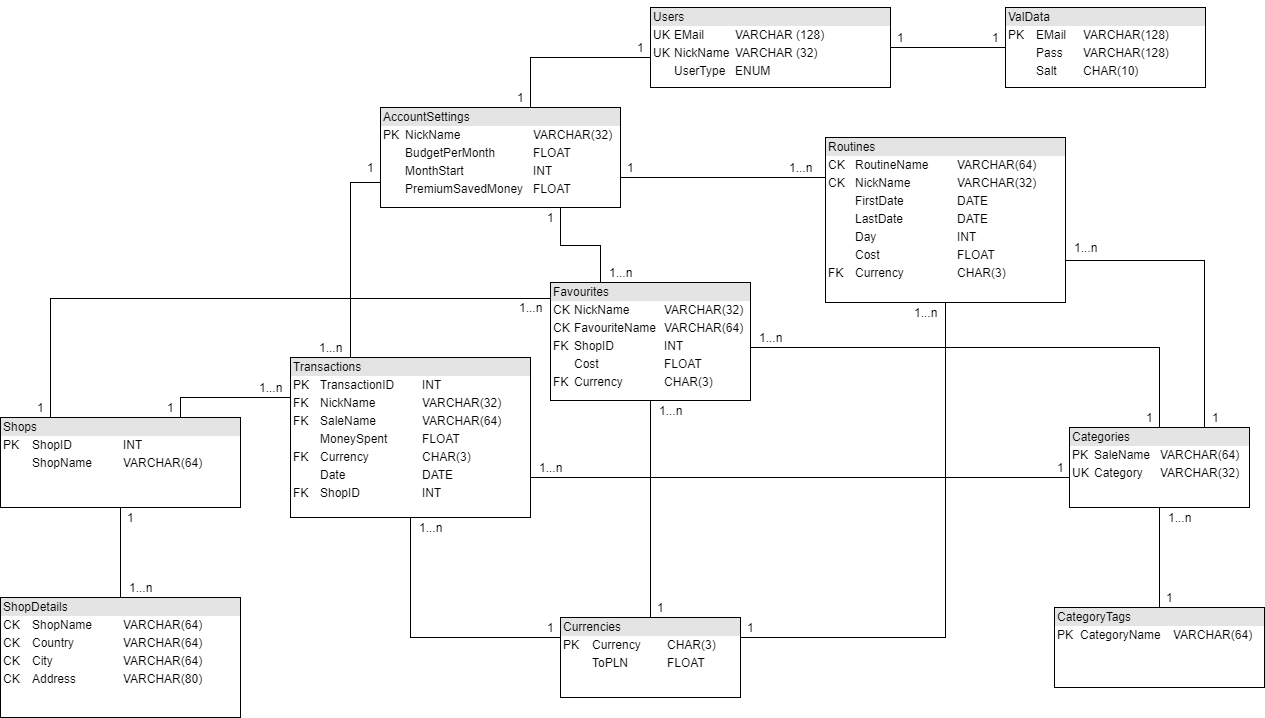
\includegraphics[width=18cm]{Project.png} 
    
    \section{Legenda do diagramu UML}
    PK - Primary Key - Klucz główny
    \\FK - Foreign Key - Klucz obcy
    \\CK - Composite Key - Klucz łączony
    \\U - Unique - Wartość unikalna
    \\
    \\Users - Przechowuje dane użytkowników
    \begin{itemize}
    \item sda
    \end{itemize}
    ValData - Przechowuje dane uwierzytelnienia użytkowników
    \\AccountSettings - Przechowuje dane o ustawieniach konta
    \\Transactions - Przechowuje rekordy transakcji użytkowników
    \\Routines (Premium) - Przechowuje dane o płatnościach stałych użytkowników Premium
    \\Favourites (Premium) - Przechowuje dane o ulubionych płatnościach użytkowników Premium
    \\Categories - Przechowuje dane o kategoriach produktów, usług podanych w transakcjach
    \\Shops - Przechowuje podstawowe dane o sklepach i miejscach świadczenia usług
    \\ShopDetails - Przechowuje szczegółowe dane o sklepach i miejscach świadczenia usług
    
    \section{Scenariusze użycia}
    Aplikacja ma duże możliwości, natomiast podane poniżej są przykładowe scenariusze jej użycia:
    \begin{enumerate}
    \item Użytkownik zakłada konto, ustala miesięczny budżet do rozdysponowania, następnie w danym miesiącu wprowadza dane o opłaconych usługach.
    \item Klient postanawia sprawdzić w jakim sklepie zakupił produkt po najniższej cenie, kiedy transakcja odbyła się ponad miesiąc wcześniej. Sprawdza historię płatności, ogranicza wyniki do produktu i sortuje po dacie.
    \item Klient zastanawia się ile miesięcznie płaci za poranną kawę, którą pije od czasu do czasu przed rozpoczęciem pracy, więc ustawia tę czynność jako ulubioną i sprawdza sumę kosztów pod koniec miesiąca.
    \item Student chce oszczędzić pewną sumę z dostępnego dla niego budżetu, a po paru miesiącach, wydać ją na zakup dobrej książki, więc włącza opcję liczenia osczędności w aplikacji.
    \item Użytkownik włącza do miesięcznych rachunków stałą płatność za Internet, abonament telefoniczny etc. W konkretnym ustalonym dniu, system odejmuje od pozostałego budżetu koszt opłacenia usługi.
    \end{enumerate}
    
    
    
% PRZYKŁADY LIST (jeśli zapamiętałeś, możesz skasować):
%
%    \begin{enumerate}
%    	\item Pierwszy podpunkt przykładowej listy numerowanej
%    	\item Drugi podpunkt przykładowej listy numerowanej
%    \end{enumerate}
%
%    \begin{enumerate}[a)]
%    	\item Pierwszy podpunkt przykładowej listy a,b,c...
%    	\item Drugi podpunkt przykładowej listy a,b,c...
%    \end{enumerate}
%
%    \begin{itemize}
%    	\item Pierwszy podpunkt przykładowej listy wypunktowanej
%    	\item Drugi podpunkt przykładowej listy wypunktowanej
%    \end{itemize}

    
\end{document}    
 
